\chapter{Sensitivity of the SuperNEMO demonstrator to the $\zeronu$}
\label{ch:sensitivity}


In this chapter, we present the SuperNEMO sensitivity to the search of $\zeronu$ decay, and the corresponding effective neutrino masses, for several isotopes.
The SuperNEMO final detector is expected to exclude $\zeronu$ half-lives up to $1.2\times 10^{26}$ y ($90\%$ CL) if $\zeronu$ decays through the exchange of a light Majorana neutrino, with a detector exposure of $500$ kg.y \cite{art:SuperNEMO2010}.
The sensitivity is given as a limit, in case we do not observe the expected signal.
In $2010$ began the demonstrator installation at the Laboratoire Souterrain de Modane.
With an exposure of $17.5$ kg.y, the demonstrator could set a limit on the $\zeronu$ process of $5.35\times 10^{24}$ y ($90\%$ CL) \cite{CalvezThesis}.

This study aims to explore the impact on the sensitivity of the presence of a magnetic field, and will participate in the final decision on the installation of the coil.
In a context of investigating the demonstrator and final detector capabilities, different internal source contamination levels are explored.
The topology of interest is the two electrons topology, and we use the $2e$ energy sum to discriminate the signal from the background events.
Thanks to SuperNEMO tracking capabilities, topological informations are exploited to improve the SuperNEMO sensitivity.



\section{Signal and background simulations}
\label{sec:sensitivity_simus}

A full simulation for the SuperNEMO demonstrator was perfomed, in order to determine the longest $\zeronu$ half-life that can be probed with SuperNEMO using the distribution of the sum of electron energies, in the case where the $\zeronu$ decay were not observed.
In the Tab.~\ref{tab:sensitivity_simulations} is summarised the expected number of signal and background events, both for the SuperNEMO demonstrator and final detector, and we present the size of Monte-Carlo simulations for each isotope.
\begin{table}[h]
  \centering
  \begin{tabular}{|c|cc|c|}
    \hline
    &\multicolumn{2}{c|}{Expected decays} & Simulated decays \\
    & Demonstrator & Final detector & \\
    \hline\hline
    $\zeronu$ ($\Tbeta = 2.5\,10^{23}$ y) & $3.6\,10^{2}$ & $1.0\,10^{4}$ & $1.0\,10^{7}$ \\
    $\twonu$ & $9.5\,10^{5}$ & $2.7\,10^{7}$ & $1.0\,10^{7}$ \\
    \Tl  & $5.5\,10^{3}$ & $1.6\,10^{5}$ & $1.0\,10^{7}$ \\
    \Bi  & $1.1\,10^{3}$ & $3.1\,10^{4}$ & $1.0\,10^{7}$ \\
    \Rn  & $1.8\,10^{5}$ & $7.2\,10^{6}$ & $1.0\,10^{7}$ \\
    \hline
  \end{tabular}
  \caption{Expected and simulated decays for different processes, both for the demonstrator ($17.5$ kg.y) and for the final detector ($500$ kg.y), assuming target background activities are reached.
    The $\Tbeta$ value is given only illustratively: the decay has never been observed, so we choose the limit on the half-life obtained with NEMO-$3$ [ref].
    Exepected number of events are given not taking into account the cut efficiencies, and in the full energy range.
    We remind the target activities: $\mathcal{A}^{\text{Tl}} = 10\,\mu$Bq.kg, $\mathcal{A}^{\text{Bi}} = 2\,\mu$Bq.kg, $\mathcal{A}^{\text{Rn}} = 0.15$ mBq.m$^{-3}$
    \label{tab:sensitivity_simulations}}
\end{table}


\subsubsection*{The $\zeronu$ signal}

In the following, the assumed underlying mechanism for the $\zeronu$ decay exist through the exchange of a light Majorana neutrino, the so-called mass mechanism (MM), as it is the most natural and widespread mechanism.
The hypotetical $\zeronu$ signal would be detected as an excess of events in the region of interest, with respect to the predicted background contamination level.
The $10^{7}$ $\zeronu$ Monte-Carlo events are generated using the DECAY$0$ software~\cite{art:decay0}.
The simulations are normalised assuming a $\Tbeta = 6.0\,10^{24}$ y half-life [citation].

\subsubsection*{Inside detector backgrounds}

In the full energy range, the allowed $\twonu$ decay stands as the dominant internal background type.
However, beyond a certain value in energy, the number of $\twonu$ events decreases very quickly, because of the energy spectrum shape.
Moreover, its contribution is reduced if the half-life increases, and is enhanced if the energy resolution is worsened.
To offset this effect, we simulated $10^{7}$ $\twonu$ decays inside the source foils, with a total energy $>2$ MeV, in addition of the normal $\twonu$ decays.
($\Ttwonu = 9.39 \pm 0.17$ (stat) $\pm 0.58$ (syst) $\times 10^{19}$ years from the NEMO-$3$ experiment~\cite{art:NEMO2018}), and we normalised the total $\twonu$ spectrum.
As described in Sec.~\ref{subsec:SNbkg_internal}, source foil contaminations by isotopes such as \Tl\ or \Bi\ constitute the principal internal backgrounds with the $\twonu$ decay.
These backgrounds are processed by the same detector simulation as the $\zeronu$ signal, using DECAY$0$.
Since internal backgrounds have very low efficiencies in the $2e$ topology, we simulated an important amount of Monte-Carlo events.

A component of the external background producing events similar to the internal background is caused by the presence of \Rn\ inside the tracking detector volume, and constitute a separate background category.
If such an decay occurs on or near a foil and appears with a $2e$ topology, it becomes hard to distinguish from a double beta decay candidate.
This isotope being distributed throughout the whole tracking detection volume, it was therefore necessary to simulate a large quantity of this isotope in the detector to maximise the amount of \Bi\ events, coming from \Rn\ decays, in the region of interest.

The target background activities detailed in Sec.~\ref{sec:SNbkg} were defined so that each background has a similar contribution to that of the $\twonu$ in the region of interest~\cite{internal:SNphysicsCase}.
We remind these nominal in Tab.~\ref{tab:real_target_act}, and give a comparison with the measured activities of the demonstrator source foils contaminations, as well as a measurement of the \Rn\ activity inside the tracker volume.
\begin{table}[h]
  \centering
  \begin{tabular}{|c|c|c|}
    \hline
    & Nominal activities & Real activities \\
    \hline\hline
    \Tl  & $10\,\mu$Bq.kg$^{-1}$ & $54\,\mu$Bq.kg$^{-1}$ \\
    \Bi  & $2\,\mu$Bq.kg$^{-1}$ & $<290\,\mu$Bq.kg$^{-1}$ \\
    \Rn  & $0.15$ mBq.m$^{-3}$ & $0.15\pm 0.02$ mBq.m$^{-3}$~\cite{conf:radon2017} \\
    \hline
  \end{tabular}
  \caption{Real and targeted nominal activities for the SuperNEMO detector.
  \label{tab:real_target_act}}
\end{table}


\subsubsection*{Outside detector backgrounds}

This background category is due to the external $\gamma$-ray flux produced by radioactive isotope decays in detector components or surrounding laboratory rocks, as well as neutron interactions in the shield and of the detector's material.
The limit on external background number of counts set by the NEMO-$3$ experiment was $<0.2$ in the $2e$ total energy range [$2.8$;$3.2$] MeV, for an exposure of $34.3$ kg·y~\cite{art:NEMO2015}.
The most notorious difference is the fact that the SuperNEMO scintillator blocks are thicker than those of NEMO-$3$.
Therefore, a gamma is less likely to cross a scintillator without interacting, and we can reject it if an interaction occurs.
As a consequence, for the same PMTs radioactivity, the gamma background rate is less important for the SuperNEMO demonstrator than for NEMO-$3$.
Moreover, radiopurity measurement for SuperNEMO PMTs allow to conclude that the total activity of SuperNEMO PMTs is better than for NEMO-$3$, for the two principal considered isotopes \Tl\ and \Bi ~\cite{docdb:perrot2017}.
Thus, it is justified to consider that all external backgrounds from outside the foil, apart from \Rn\ in the tracking volume, are expected to be negligible, and were not simulated.\\

We select only events matching the $2e$ toplogy.
A reconstructed particle is tagged as an electron if it has a negatively curved track with a vertex on the source foils and an associated calorimeter hit.
All these represent what we call \emph{the first order cuts}.
In the following we present an optimisation of the event selection that have been set up to maximise the signal over background ratio.

%% \begin{itemize}
%% \item Justifier bdf externe avec article nemo3 (plus diff roi et meilleure eff)
%% \item The dominant two neutrino $\twonu$ background and the background due to foil contaminations were normalised assuming a demonstrator exposure of $17.5$ kg.y.
%% \item The total energy brought by the two electrons is a continuum presenting a reduced number of events in the region of interest, due to electron energy losses before reaching the calorimeter (mainly inside the dense source material, as well as inside the wire chamber).
%% \end{itemize}


\section{Optimisation of event selection}
\label{sec:sensitivity_ev_selection}

Most of the double beta experiments are only sensitive to the total electron energy sum.
SuperNEMO, coupling tracking and calorimetry technologies, has the ability to consider individually the two emitted electrons, and to evaluate wether the two particles were emitted simultaneously from the same vertex or not.
To allow the selection of $\zeronu$ signal events while rejecting a high proportion of background events, topological cuts have been set up, in addition with the basical first order cuts described above.
\begin{itemize}
\item \Pint\ $>4\%$:\\
  The internal probability, based on time-of-flight (TOF) computation, is detailed in Sec.~\ref{subsec:internal_prob}.
  The chosen level insures that non simultaneous events are rejected.
\item $\Delta y < 60$ mm and $\Delta z < 70$ mm:\\
  The two reconstruted vertices on source foils should not be separated by more than $60$ mm horizontally, and by more than $70$ mm vertically, to maximise the selection of two electrons emitted at the same spot.
\end{itemize}
These cuts follow the NEMO-$3$ analysis on the external background rejection, whose effectiveness were lately confirmed for the SuperNEMO demonstrator~\cite{docdb:calvez2014}.
First order and topological cuts have an efficiency of selection that differs for each decays.
These efficiencies are presented in Tab.~\ref{tab:selections_eff}.
\begin{table}[h]
  \centering
  \begin{tabular}{|c|c|c|c|}
    \hline
    & First order cuts & Internal probability & Vertex distance  \\
    \hline\hline
    $\zeronu$  &  & & \\
    $\twonu$  &  & & \\
    \Tl  &  & & \\
    \Bi  &  & & \\
    \Rn  &  & & \\
    \hline
  \end{tabular}
  \caption{Selection efficiencies for first order cuts and topological cuts.
  \label{tab:selections_eff}}
\end{table}
Topological cuts are designed to reject events where the two electrons are not emitted simultaneously, or from the same location on the source foil, and hence decreases the number of expected events for all the backgrounds but especially for Radon.
As explained in Sec.~\ref{sec:sensitivity_simus}, the Radon events are not emitted from the source, but mainly from the tracker wires.
The internal probability and vertices separation can therefore help discriminate such events from signal events.

We present the total energy spectra for each simulated process, after event selection, in Fig.~\ref{fig:sensitivity_energy_spectra}.
\begin{figure}[h]
\centering
\begin{subfigure}[t]{0.48\textwidth}
  \centering
  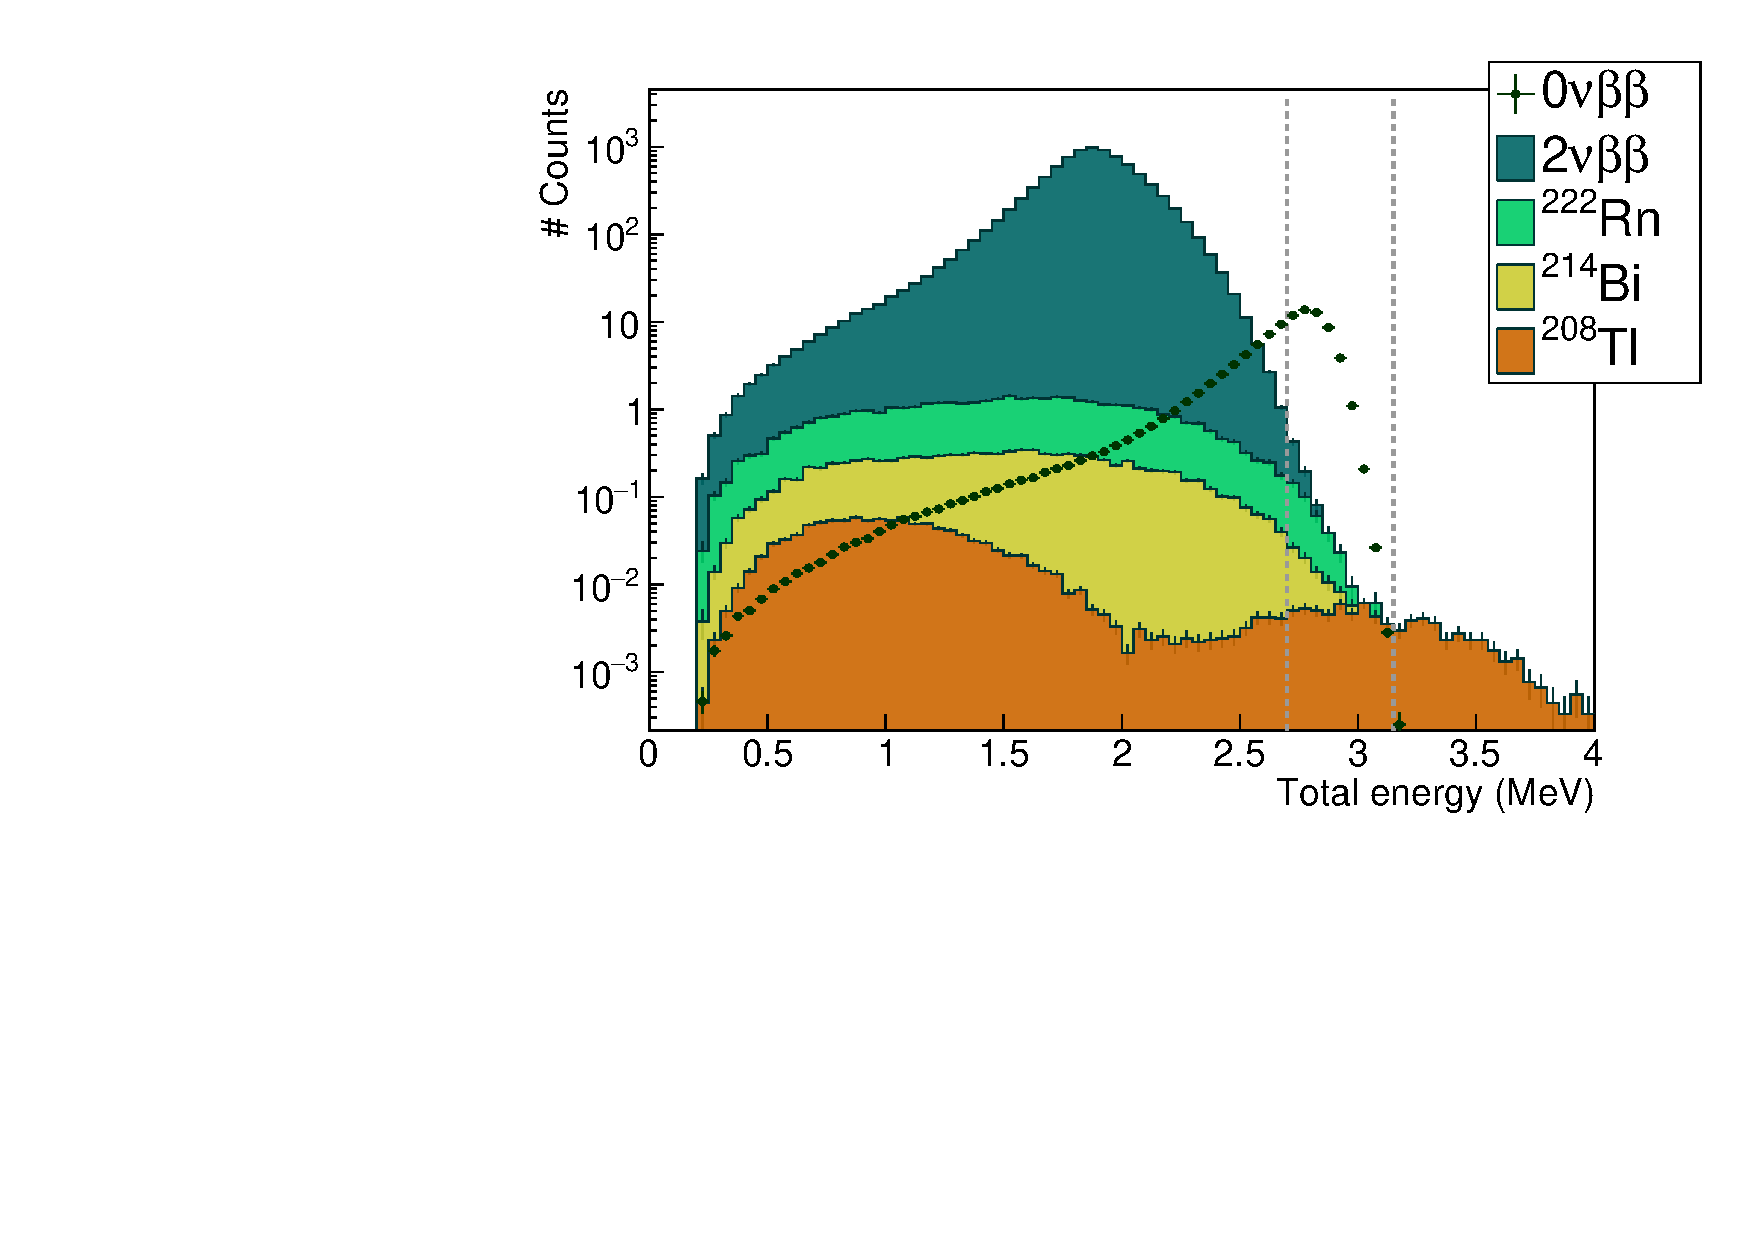
\includegraphics[width=1.1\textwidth]{Sensitivity/fig_sensitivity/energy_spectrum_with_B_82Se.pdf}
  \captionsetup{justification=centering}
  \caption{
    \label{subfig:sensitivity_energy_spectra_full}}
\end{subfigure}
\hfill
\begin{subfigure}[t]{0.48\textwidth}
  \centering
  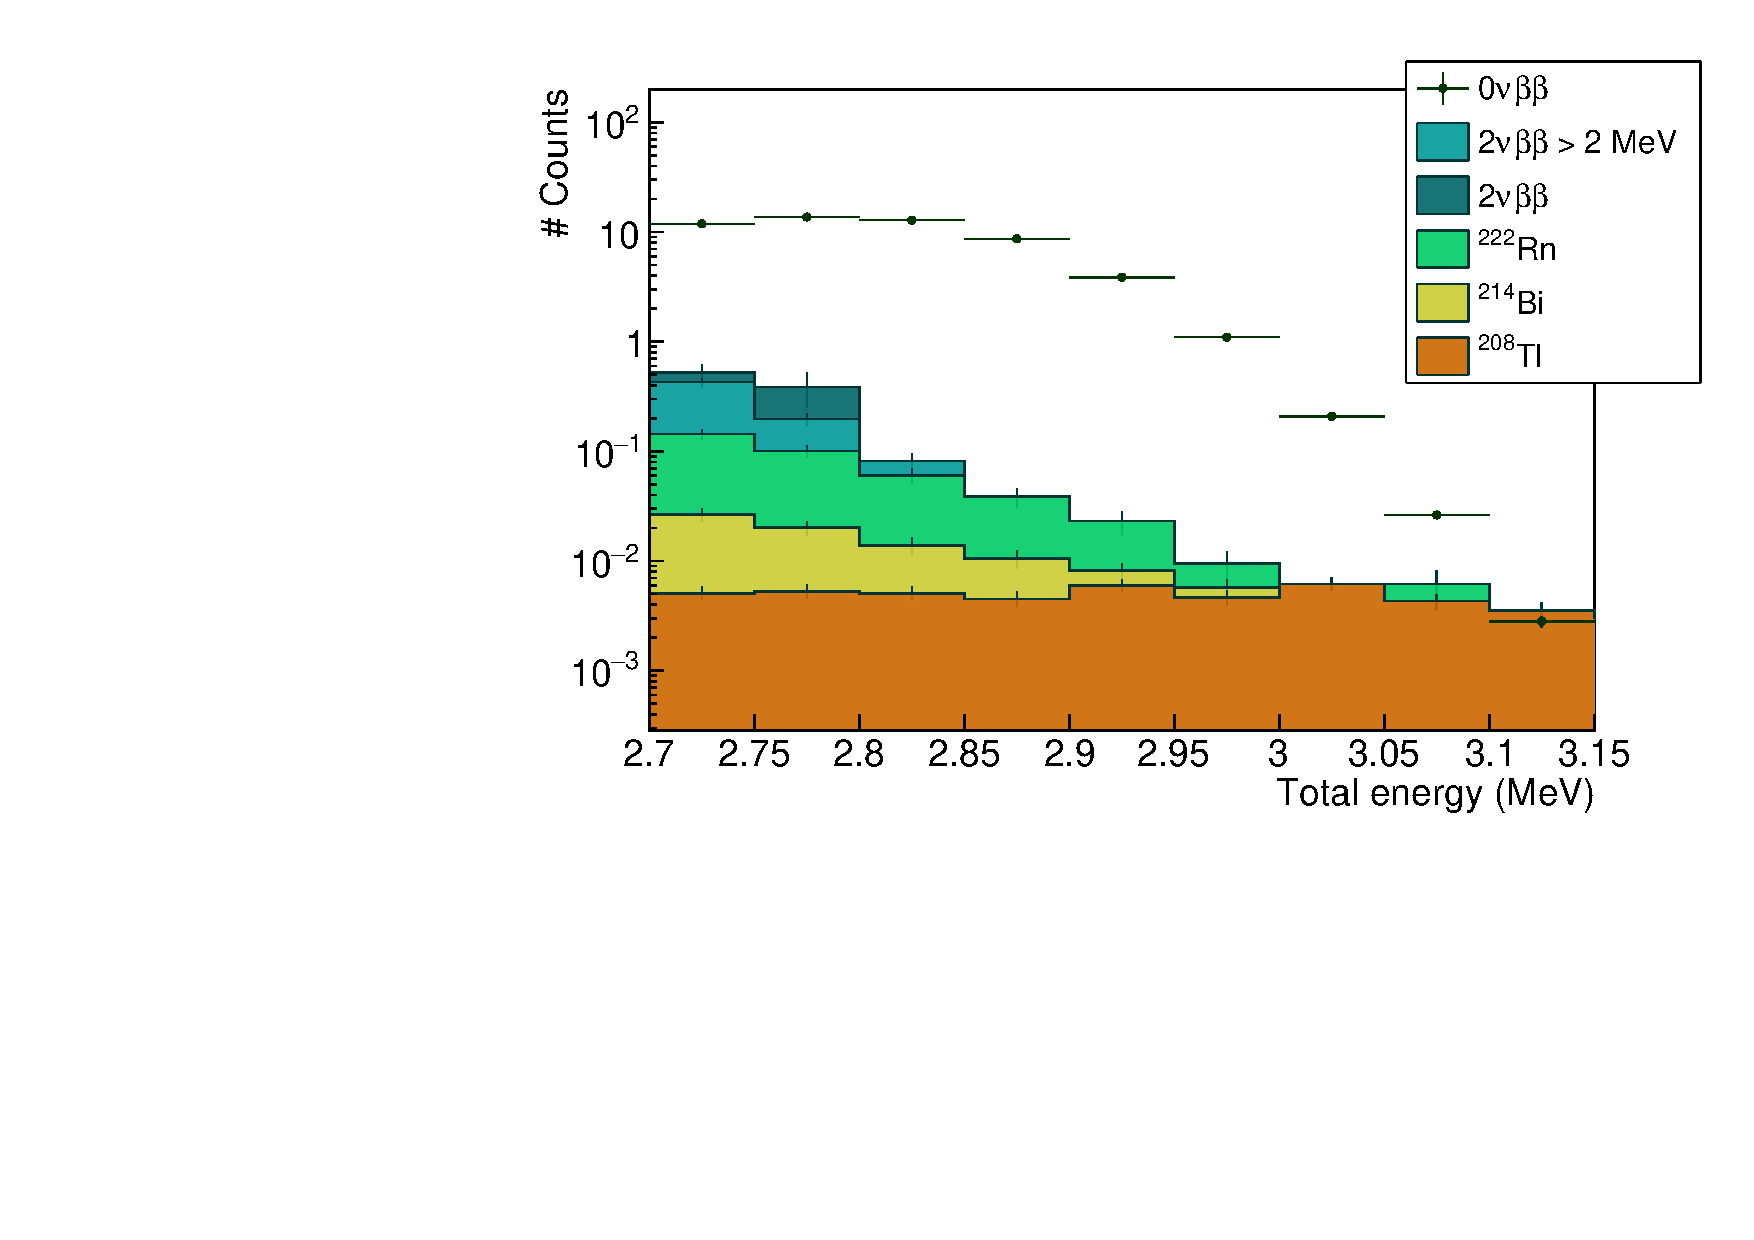
\includegraphics[width=1.1\textwidth]{Sensitivity/fig_sensitivity/energy_spectrum_with_B_82Se_zoom.pdf}
  \captionsetup{justification=centering}
  \caption{
    \label{subfig:sensitivity_energy_spectra_zoom}}
\end{subfigure}
\caption{Total energy spectra for the $\zeronu$ signal and main backgrounds, for the full energy range (a) and for the [$2.7$;$3.2$] MeV energy range (b).
  \label{fig:sensitivity_energy_spectra}}
\end{figure}
% The total number of events for each decay represent the amount of selected $2e$ topologies.
The $\zeronu$ spectrum is peaked around $2.8$ MeV, as the available energy $\Qbb = 2.99$ MeV is degraded by electron energy losses before reaching the calorimeter (mainly inside the dense source material, as well as inside the wire chamber), explaining the asymetric energy distribution.
% The progeny of \Rn\ produces $\gamma$-rays and $\beta$ decays accompanied by internal conversion (IC), Møller or Compton scattering, the dominant mechanism being the first one.
\Bi\ being one of the descendents of \Rn, their energy distributions follow the same variations, exept that a high part af \Rn\ events inside the tracker have been rejected by the topological cuts.
The \Tl\ energy distribution reveals the $2.6$ MeV gamma internal conversion emitted after $\beta^{-}$ \Tl\ disintegrations.

In the following section, we give informations about the expeted number of background events, especially in the region of interest.

\section{Expected number of background events and optimisation of the region of interest}

As the two electrons energy sum for the possible $\zeronu$ is a peak (unlarged by electron energy losses and calorimeter energy resolution), it is interesting to constraint the $\zeronu$ decay searches to a given energy range, the so-called \emph{region of interest} (ROI).
In the following, we expose how the search for the best limit on $\Tbeta$ is a guid to determine the best ROI.
%The optimisation of this energy window consists of cutting the full energy range in several sub-ranges, and compute the selection efficiencies for all energy sub-ranges.

For a given energy range, the $\zeronu$ half-life depends on the signal detection efficiency $\epsilon$ in this energy window, on the number of excluded signal events $N_{\text{exclus}}$, as well as on the source isotope nature and the detector's exposure $m\times t$, following
\begin{equation}
  \Tbeta > \frac{\mathcal{N}_{\text{A}}\log{2}}{M}\times \frac{\epsilon\times m\times t}{N_{\text{exclus}}}\,,
\end{equation}
with $\mathcal{N}_{\text{A}}$ the Avogadro number and $M$ the source isotope's molar mass.
The half-life is given as a limit, in case we do not observe the expected signal.
In order to evaluate $N_{\text{exclus}}$, and later the demonstrator's sensitivity to the $\zeronu$ decay, we must determine the number of background events occuring in the region of interest.
This calculation, for a given energy window, differs with the background type.
\begin{itemize}
\item The $\twonu$ background\\
  The number of $\twonu$ events $N_{2\nu}$ depends, in addition to the exposure, on the number of atoms composing the source foils, on the $\twonu$ decay half-life $\Ttwonu$, and on $\epsilon_{2\nu}$ the selection efficiency for the $\twonu$ process, as
  \begin{equation}
    N_{2\nu} = \frac{\mathcal{N}_{\text{A}}\log{2}}{M}\times\frac{\epsilon_{2\nu}\times m\times t}{\Ttwonu}\,.
  \end{equation}
\item Natural radioactive internal backgrounds (\Tl\ and \Bi)\\
  Considering $A_{\text{int}}$ as the internal background activities, and $\epsilon_{\text{int}}$ their selection efficiencies in a given energy window, the number of background events emitted from the source is
  \begin{equation}
    N_{\text{int}} = A_{\text{int}}\epsilon_{\text{int}}\times m\times t\,.
  \end{equation}
\item Radon background\\
  The same way, we can define the number of radon events occuring in the whole tracker volume $V$ as
  \begin{equation}
    N_{\text{Rn}} = A_{\text{Rn}}\epsilon_{\text{Rn}}\times V\times t\,.
  \end{equation}
\end{itemize}
The efficiency spectra, computed by comparing the number of selected events to the number of Monte Carlo events, are presented in Fig.~\ref{fig:sensitivity_efficiency_spectra}.
\begin{figure}[h]
  \centering
  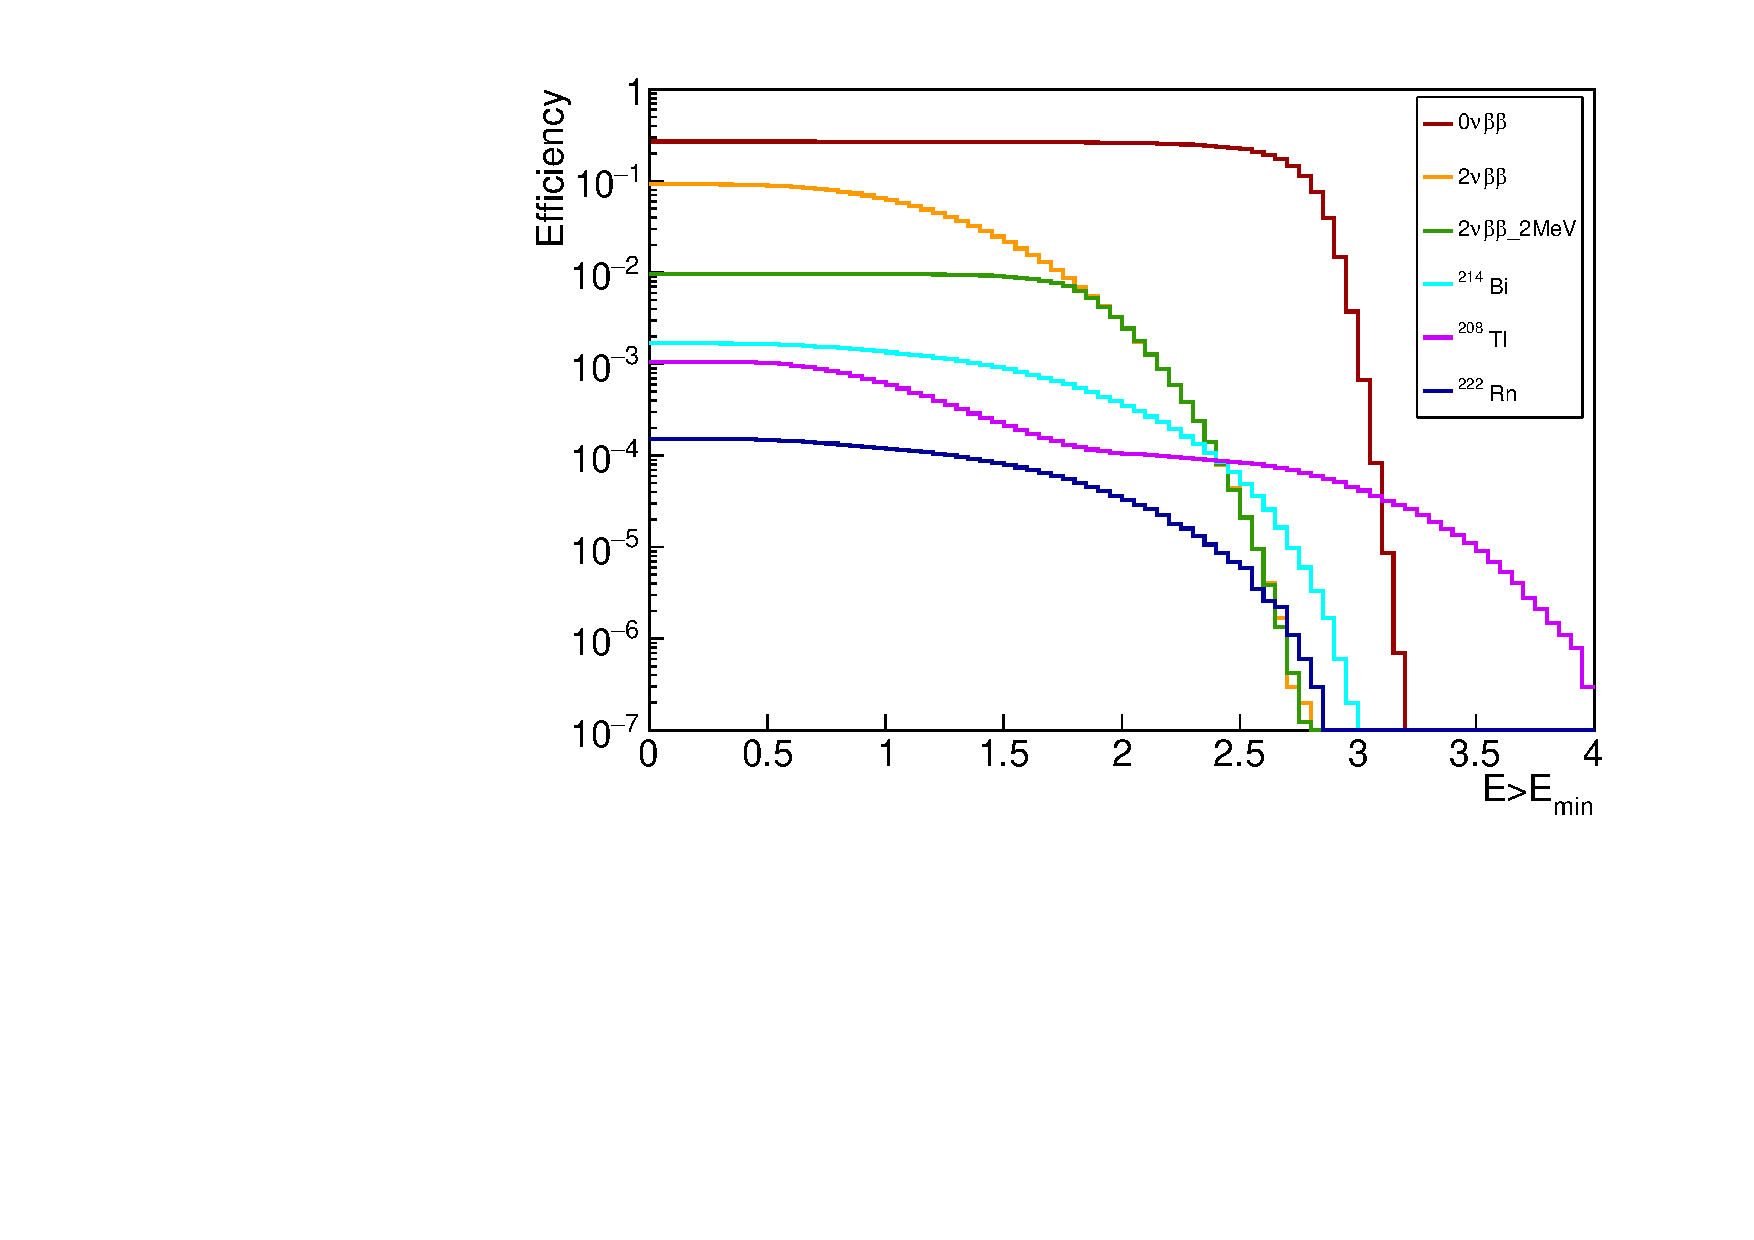
\includegraphics[width=1.1\textwidth]{Sensitivity/fig_sensitivity/efficiency_spectrum_with_B_82Se.pdf}
  \caption{Efficiency spectra for $\text{E}>\text{E}_{\text{min}}$, for the $\zeronu$ signal and for the main backgrounds.
    \label{fig:sensitivity_efficiency_spectra}}
\end{figure}
These are cumulated efficiencies, and given as a function of $E>E_{\text{min}}$.


Tab.~\ref{tab:2e_expected_counts} sums up the expected number of counts in the full energy range as well as in the region of interest.
\begin{table}[h]
  \centering
  \begin{tabular}{|c|c|c|}
    \hline
    & Full energy range & [$2.75$;$2.85$] MeV \\
    \hline\hline
    $\zeronu$  & $2.7\,10^{6}$ & $9.5\,10^{-2}$ \\
    $\twonu$  & $9.1\,10^{5}$ & $1.1\,10^{-1}$ \\
    \Tl  & $1.7\,10^{4}$ & $9.9^{-3}$ \\
    \Bi  & $1.1\,10^{4}$ & $2.7\,10^{-2}$ \\
    \Rn  & $1.1\,10^{4}$ &  \\
    \hline
  \end{tabular}
  \caption{Expected number of counts for the full energy range and for the region of interest.
  \label{tab:2e_expected_counts}}
\end{table}

Once computed, the efficiency of selection helps finding the number of background events expected, for $\text{E}>\text{E}_{\text{min}}$, presented in Fig.~\ref{fig:sensitivity_Nbkg_spectra}.
\begin{figure}[h]
  \centering
  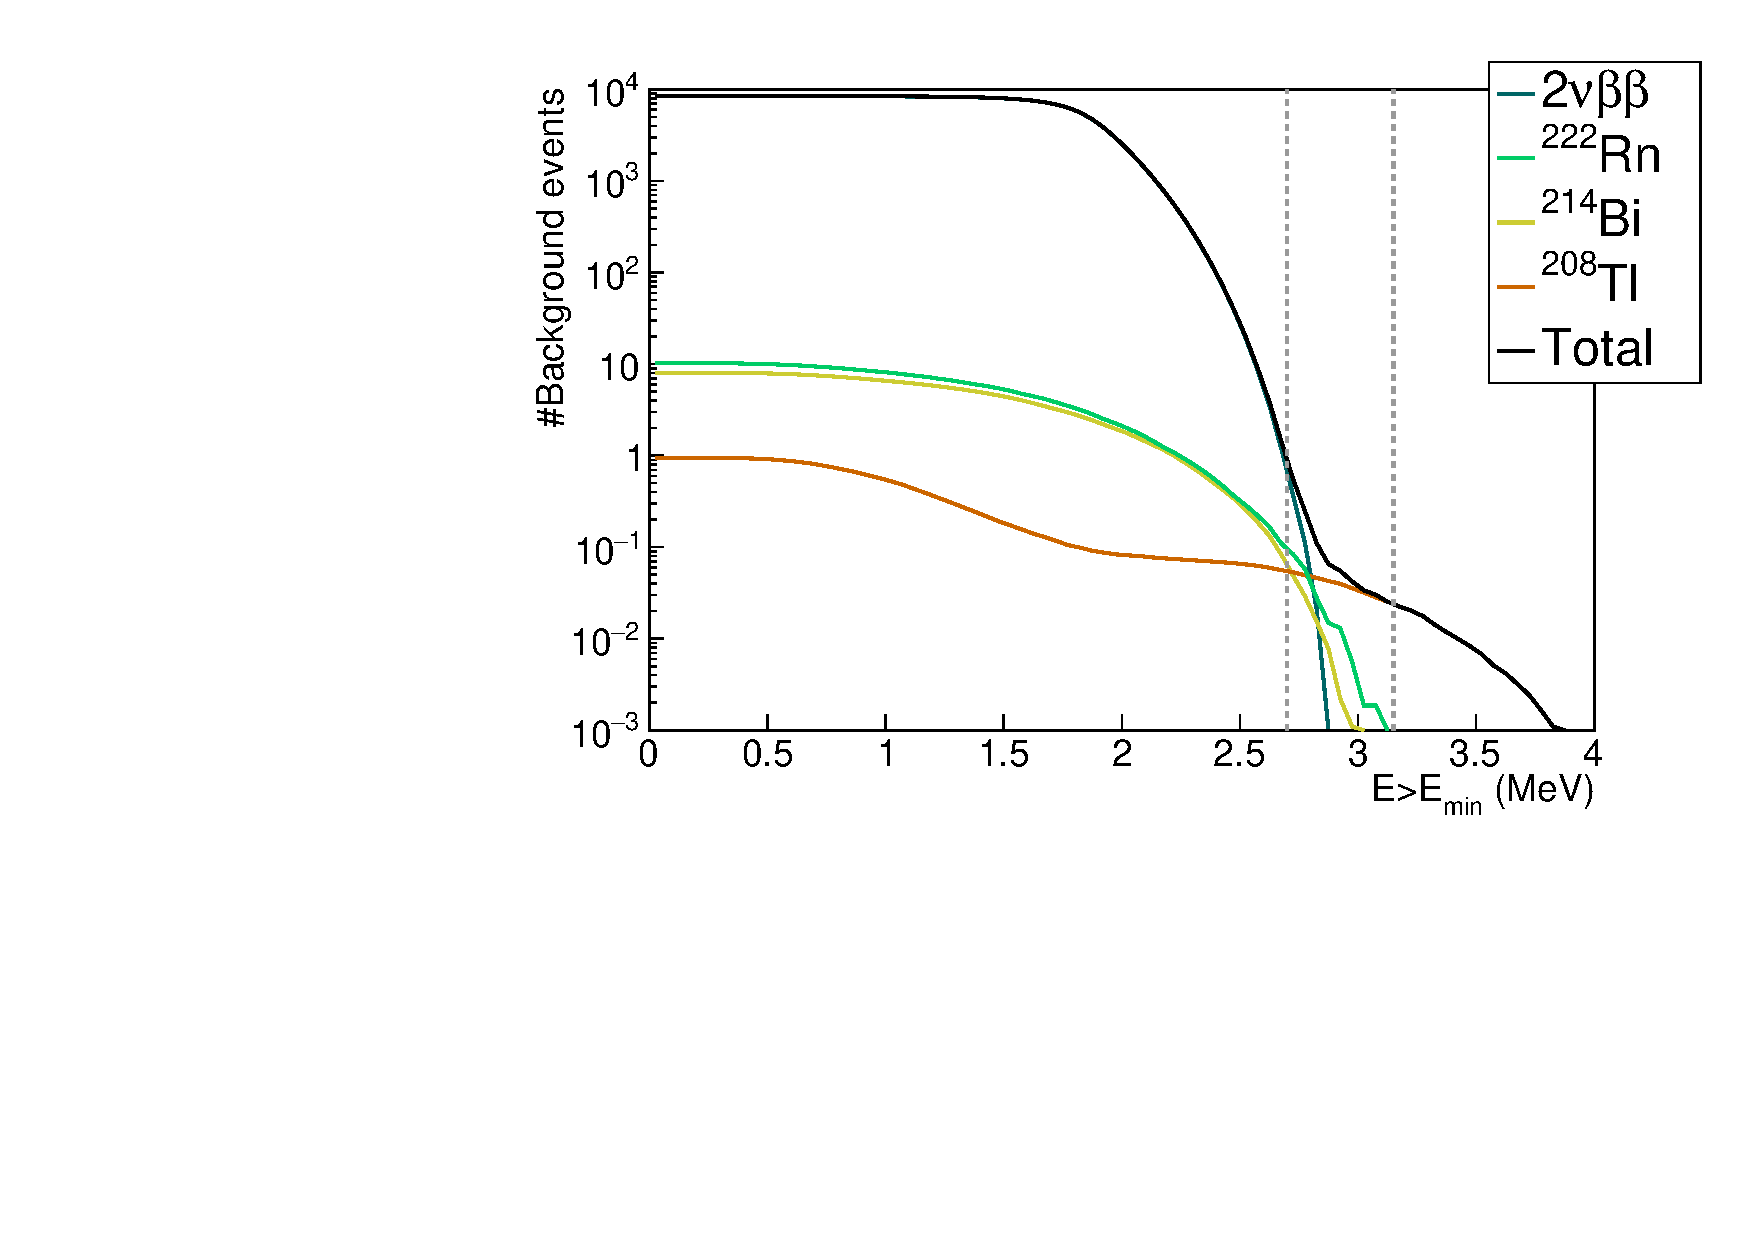
\includegraphics[width=1.1\textwidth]{Sensitivity/fig_sensitivity/Nbackground_spectrum_with_B_82Se.pdf}
  \caption{Expected number of background events, for $\text{E}>\text{E}_{\text{min}}$.
    \label{fig:sensitivity_Nbkg_spectra}}
\end{figure}


\section{Demonstrator sensitivity}

\begin{itemize}
\item Résultats $B=0$, avec activités nominales, puis avec activités caca
\item Influence des quantités de contaminations sur la sensibilité
\end{itemize}

\subsection{avec B}
Parler du champ non uniforme/attenuation
ROI optimization: avec variation coupure énergie\\

\subsection{sans B}
avec variation coupure énergie\\

\subsection{Champ mappé}


\section{HyperNEMO}
results for $500$kg.y exposure

\section{Other isotopes}

distribution t1/2 avec différents échantillons de simus (17.5 kg.y)

\section{Conclusion}
\begin{itemize}
\item Etude plus générale avec bkg externe+lab (reprendre chiffres NEMO3) + neutrons (cf NEMO3)
\item Plot général récap tous résultats
\item delayed cells->improvement, cf NEMO 3
\end{itemize}
